\documentclass[10pt]{beamer}
\usepackage{amsmath}
\usepackage{mathtools}
\usepackage{multimedia}
\usepackage{hyperref}
\usefonttheme{professionalfonts} % using non standard fonts for beamer
\usefonttheme{serif} % default family is serif
%\documentclass[12pt]{beamerthemeSam.sty}
\usepackage{epsf}
%\usepackage{pstricks}
%\usepackage[orientation=portrait,size=A4]{beamerposter}
\geometry{paperwidth=160mm,paperheight=120mm}
%DT favorite definitions
\def\LL{\left\langle}	% left angle bracket
\def\RR{\right\rangle}	% right angle bracket
\def\LP{\left(}		% left parenthesis
\def\RP{\right)}	% right parenthesis
\def\LB{\left\{}	% left curly bracket
\def\RB{\right\}}	% right curly bracket
\def\PAR#1#2{ {{\partial #1}\over{\partial #2}} }
\def\PARTWO#1#2{ {{\partial^2 #1}\over{\partial #2}^2} }
\def\PARTWOMIX#1#2#3{ {{\partial^2 #1}\over{\partial #2 \partial #3}} }

\def\rightpartial{{\overrightarrow\partial}}
\def\leftpartial{{\overleftarrow\partial}}
\def\diffpartial{\buildrel\leftrightarrow\over\partial}
\def\BS{\bigskip}
\def\BC{\begin{center}}
\def\EC{\end{center}}
\def\BN{\begin{enumerate}}
\def\EN{\end{enumerate}}
\def\BI{\begin{itemize}}
\def\EI{\end{itemize}}
\def\BE{\begin{displaymath}}
\def\EE{\end{displaymath}}
\def\BEA{\begin{eqnarray*}}
\def\EEA{\end{eqnarray*}}
\def\BNEA{\begin{eqnarray}}
\def\ENEA{\end{eqnarray}}
\def\EL{\nonumber\\}

\newcommand{\etal}{{\it et al.}}
\newcommand{\gbeta}{6/g^2}
\newcommand{\la}[1]{\label{#1}}
\newcommand{\ie}{{\em i.e.\ }}
\newcommand{\eg}{{\em e.\,g.\ }}
\newcommand{\cf}{cf.\ }
\newcommand{\etc}{etc.\ }
\newcommand{\atantwo}{{\rm atan2}}
\newcommand{\Tr}{{\rm Tr}}
\newcommand{\dt}{\Delta t}
\newcommand{\op}{{\cal O}}
\newcommand{\msbar}{{\overline{\rm MS}}}
\def\chpt{\raise0.4ex\hbox{$\chi$}PT}
\def\schpt{S\raise0.4ex\hbox{$\chi$}PT}
\def\MeV{{\rm Me\!V}}
\def\GeV{{\rm Ge\!V}}

%AB: my color definitions
%\definecolor{mygarnet}{rgb}{0.445,0.184,0.215}
%\definecolor{mygold}{rgb}{0.848,0.848,0.098}
%\definecolor{myg2g}{rgb}{0.647,0.316,0.157}
\definecolor{A}{rgb}{1.0,0.3,0.3}
\definecolor{B}{rgb}{0.0,1.0,0.0}
\definecolor{C}{rgb}{1.0,1.0,0.0}
\definecolor{D}{rgb}{0.5,0.5,1.0}
\definecolor{E}{rgb}{0.7,0.7,0.7}
\definecolor{abtitlecolor}{rgb}{1.0,1.0,1.0}
\definecolor{absecondarycolor}{rgb}{0.0,0.416,0.804}
\definecolor{abprimarycolor}{rgb}{1.0,0.686,0.0}
\definecolor{Red}           {rgb}{1,0.4,0.4}
\definecolor{Grey}          {cmyk}{.7,.7,.7,0}
\definecolor{Blue}          {cmyk}{1,1,0,0}
\definecolor{Green}         {cmyk}{1,0,1,0}
\definecolor{Brown}         {cmyk}{0,0.81,1,0.60}
\definecolor{Silver}        {rgb}{0.95,0.9,1.0}
\definecolor{Sky}           {rgb}{0.07,0.0,0.2}
\definecolor{Darkbrown}     {rgb}{0.4,0.3,0.2}
\definecolor{40Gray}        {rgb}{0.4,0.4,0.5}
\usetheme{Madrid}


\setbeamercolor{normal text}{fg=Silver,bg=Sky}

%AB: redefinition of beamer colors
%\setbeamercolor{palette tertiary}{fg=white,bg=mygarnet}
%\setbeamercolor{palette secondary}{fg=white,bg=myg2g}
%\setbeamercolor{palette primary}{fg=black,bg=mygold}
\setbeamercolor{title}{fg=abtitlecolor}
\setbeamercolor{frametitle}{fg=abtitlecolor}
\setbeamercolor{palette tertiary}{fg=white,bg=Darkbrown}
\setbeamercolor{palette secondary}{fg=white,bg=absecondarycolor}
\setbeamercolor{palette primary}{fg=white,bg=40Gray}
\setbeamercolor{structure}{fg=abtitlecolor}

\setbeamerfont{section in toc}{series=\bfseries}

%AB: remove navigation icons
\beamertemplatenavigationsymbolsempty
\title[The celestial sphere]{
  \textbf {The stars and the Earth}
}

\author [Astronomy 101]{Astronomy 101\\Syracuse University, Fall 2021\\Walter Freeman}

\date{\today}

\begin{document}



\frame{\titlepage}


\frame{\frametitle{\textbf{The celestial sphere of the stars}}
\large
``I know that I am mortal by nature and ephemeral, but when I trace at my pleasure the windings to and fro of the heavenly bodies, I no longer touch earth with my feet. I stand in the presence of Zeus himself and take my fill of ambrosia.''

\begin{flushright}--Claudius Ptolemy, from the {\it Almagest} (c. 150 CE)\end{flushright}
\BC
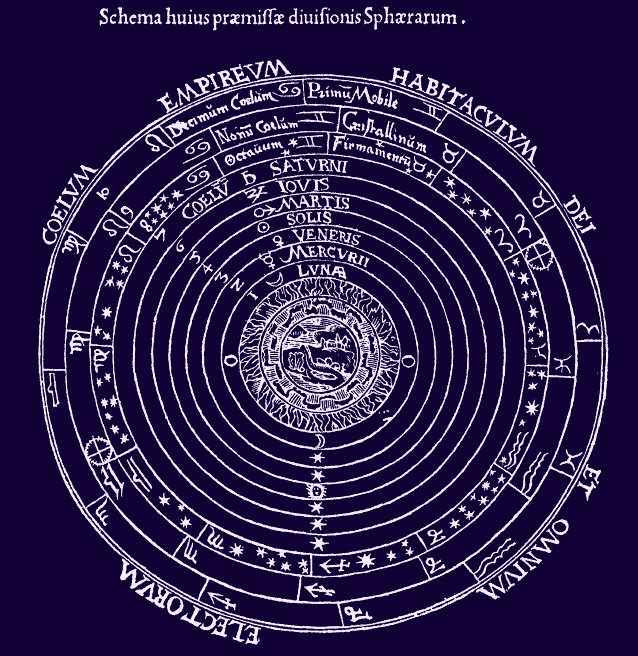
\includegraphics[width=0.4\textwidth]{sphere-medieval.png}\EC


\large


``Ooh, the wheel in the sky keeps on turning // I don't know where I'll be tomorrow...''

\begin{flushright}--Journey, ``Wheel in the Sky'' (1978)\end{flushright}


}


\frame{\frametitle{\textbf{Some announcements}}
\Large
If you missed class Tuesday:
\BI
\item{Course website: \url{walterfreeman.github.io/ast101/}}
\item{The syllabus, exercises, homework, readings, etc. are all there} 
\item Use the invite link there to join the Discord server if you wish
\item{Email for information: wafreema@syr.edu}
\item{Extra colored cards will be available each class, but they cost us a bit
of money, so try to bring yours}
\item{Prelabs have been printed and put in the Physics Clinic}
\item Having trouble installing Stellarium on your Mac? See the website for details.
\EI
}



\frame{\frametitle{\textbf{Some announcements}}
\Large

Office hours:

\BI
\item Wednesday, 2-4 PM
\item Friday, 10-12 AM
\item Subject to change occasionally when people more important than me schedule meetings I have to be at
\pause
\BS
\item I am not very important :(

\EI
}

\frame{\frametitle{\textbf{Some announcements}}
\Large
Lab section changes are tricky because things are very full. We can't run lab sections over capacity;
there is physically no room.

\bigskip
\bigskip
\bigskip

I can't do anything to override this or help you swap sections. If you need to swap sections,
you can do it on MySlice. 

\bigskip
\bigskip
\bigskip
If you sometimes come to the other {\it lecture} section than the one you signed up for, we won't probably even notice. Feel free to do this once in a while.

}

\frame{\frametitle{\textbf{Where does science start?}}
	\large
We will study the nature of science in depth later in our course.

\BS

The most fundamental property of science: {\bf \color{A}empiricism}.

\BS

Empiricism means that the {\color{B}highest authority in science} isn't what you think, or what you calculate, or what an expert says: it's what you {\color{C}observe}.

\BS\pause

It means you shouldn't trust anything I say about the night sky just because I'm a professor; it means that we have to base things on {\it data}.

\BS\pause

... so let's go look at the stars! Off to the Quad, right?

\BS\pause

... okay, let's wait until night. How well can we see the stars in the Quad at night?

\BS\pause
\BC
\url{https://youtu.be/85pRKD9EVqQ}
\EC
}



\frame{\frametitle{\textbf{The night sky and the celestial sphere: overview}}
\Large
\BI
\item{What's the night sky look like?}
\item{How have we affected the night sky?}
\item{How does the sky move each night?}
\BI
\item{The celestial-sphere model}
\item{Why it works, and when it doesn't}
\item{The first {\it Lecture Exercise}}
\EI
\EI
}



\frame{\frametitle{\textbf{Light pollution}}
\centerline{\large What do you think about this picture?} 

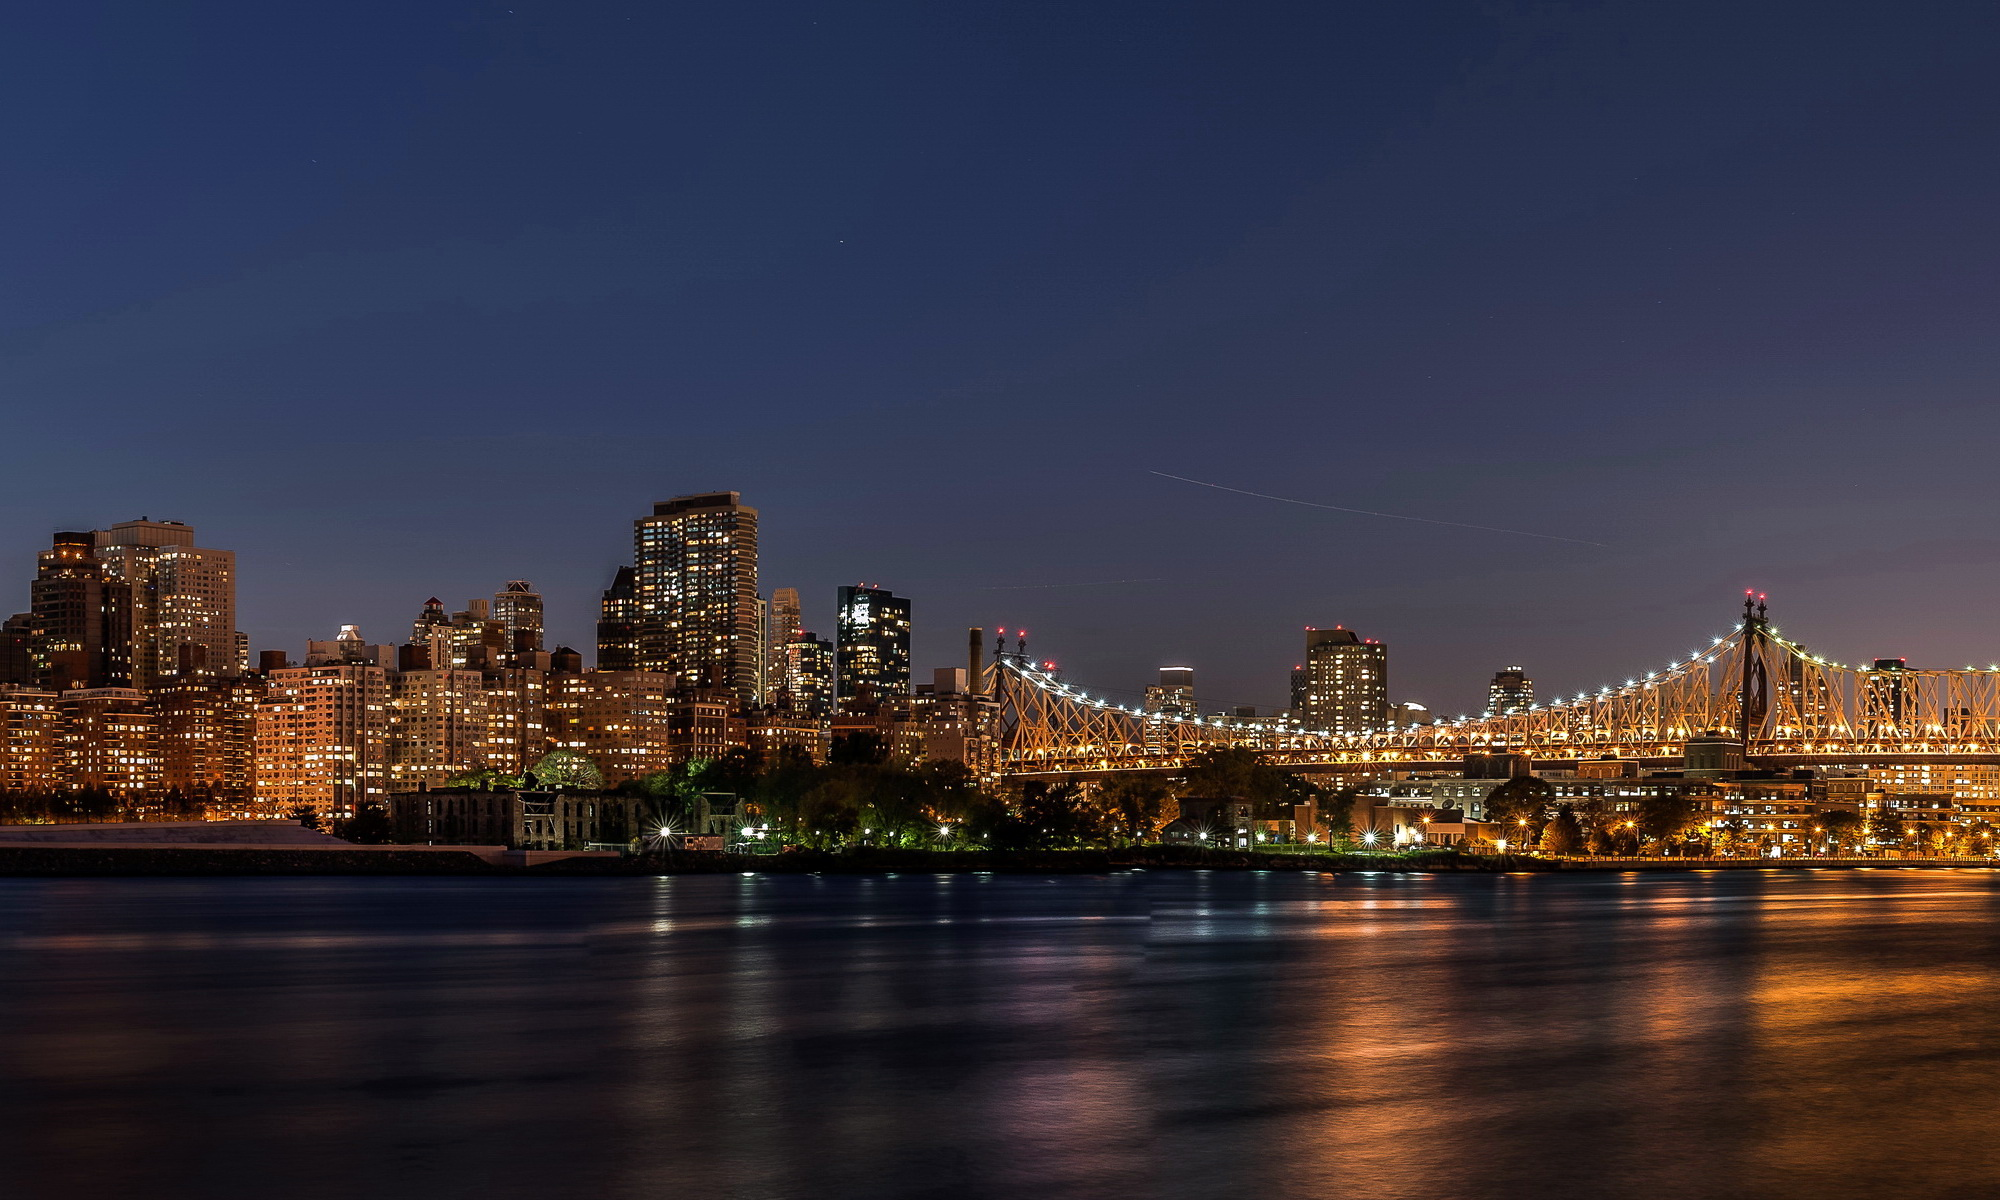
\includegraphics[width=\textwidth]{nyc-skyline.jpg}

}

\frame{\frametitle{\textbf{Light pollution}}
\centerline{\large This is what we could have instead!} 

\begin{center}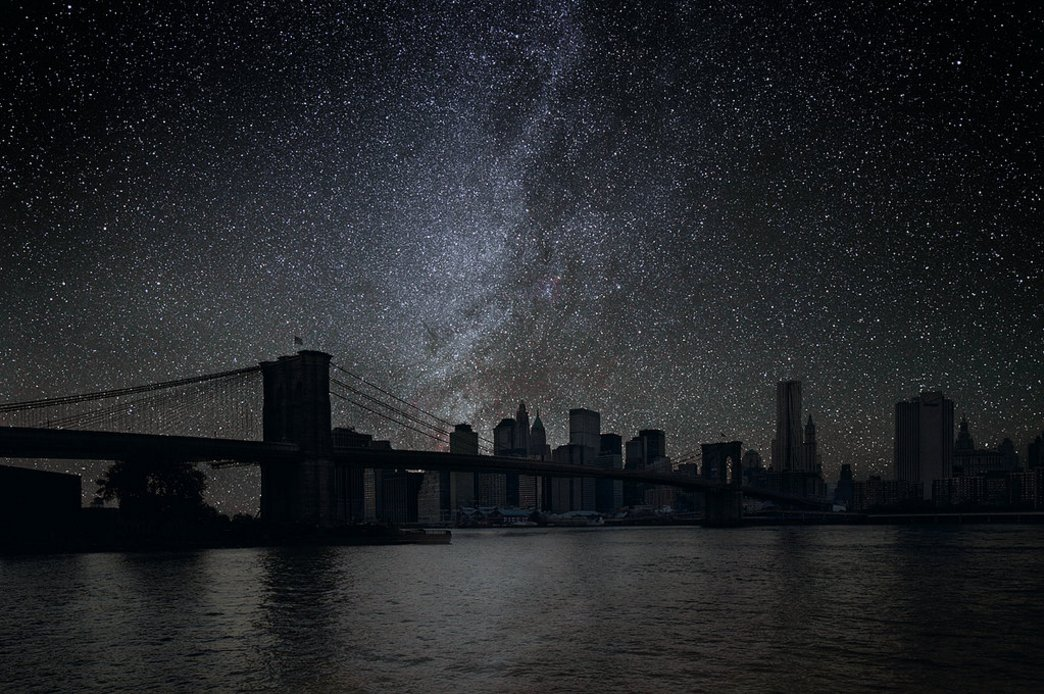
\includegraphics[width=0.92\textwidth]{nyc-skyline-dark.jpg}

\small \it (Thierry Cohen, published in the {\rm New York Times})
\bigskip
\bigskip
\bigskip

\end{center}
}

\frame{\frametitle{\textbf{Alamut, Iran}}
\BC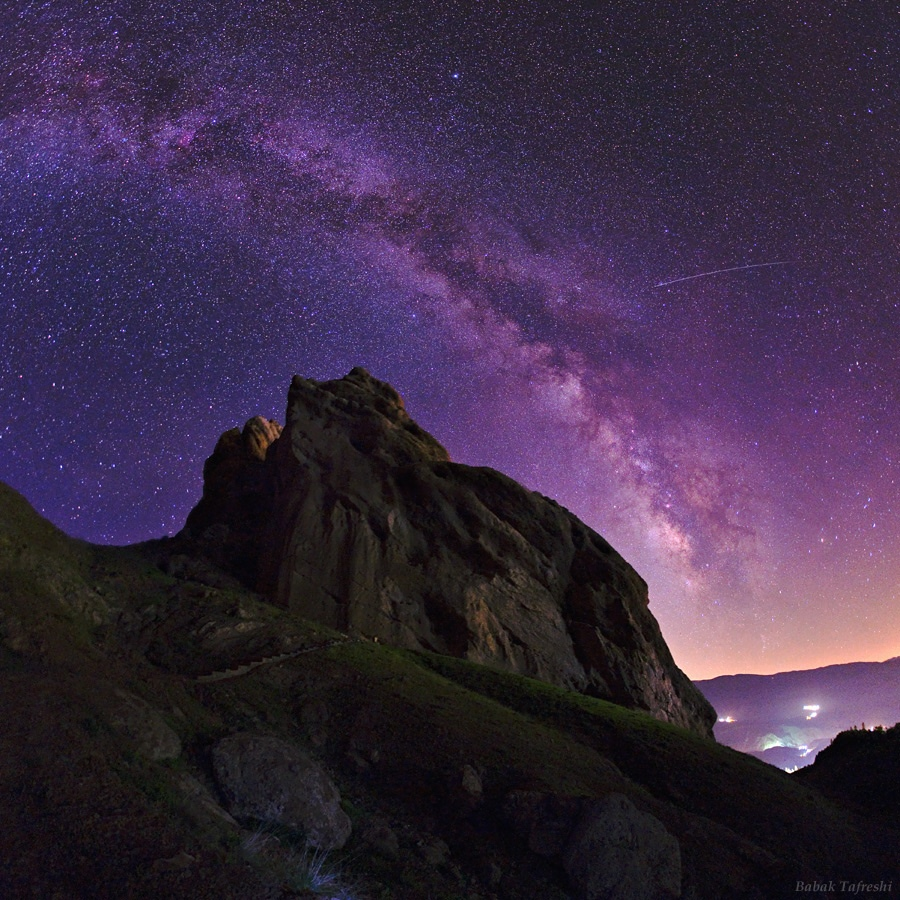
\includegraphics[width=0.6\textwidth]{alamut-babak.jpg}\EC
\small{Photo by Babek Tafreshi. Alamut was the home of Nasir al-Din al-Tusi, the first to surmise that the Milky Way was made of many stars in the $13^{\rm th}$ century. The glow is light pollution from Tehran, 100 km away.}
}

%\frame{\frametitle{\textbf{Canyonlands National Park, Utah}}
%\BC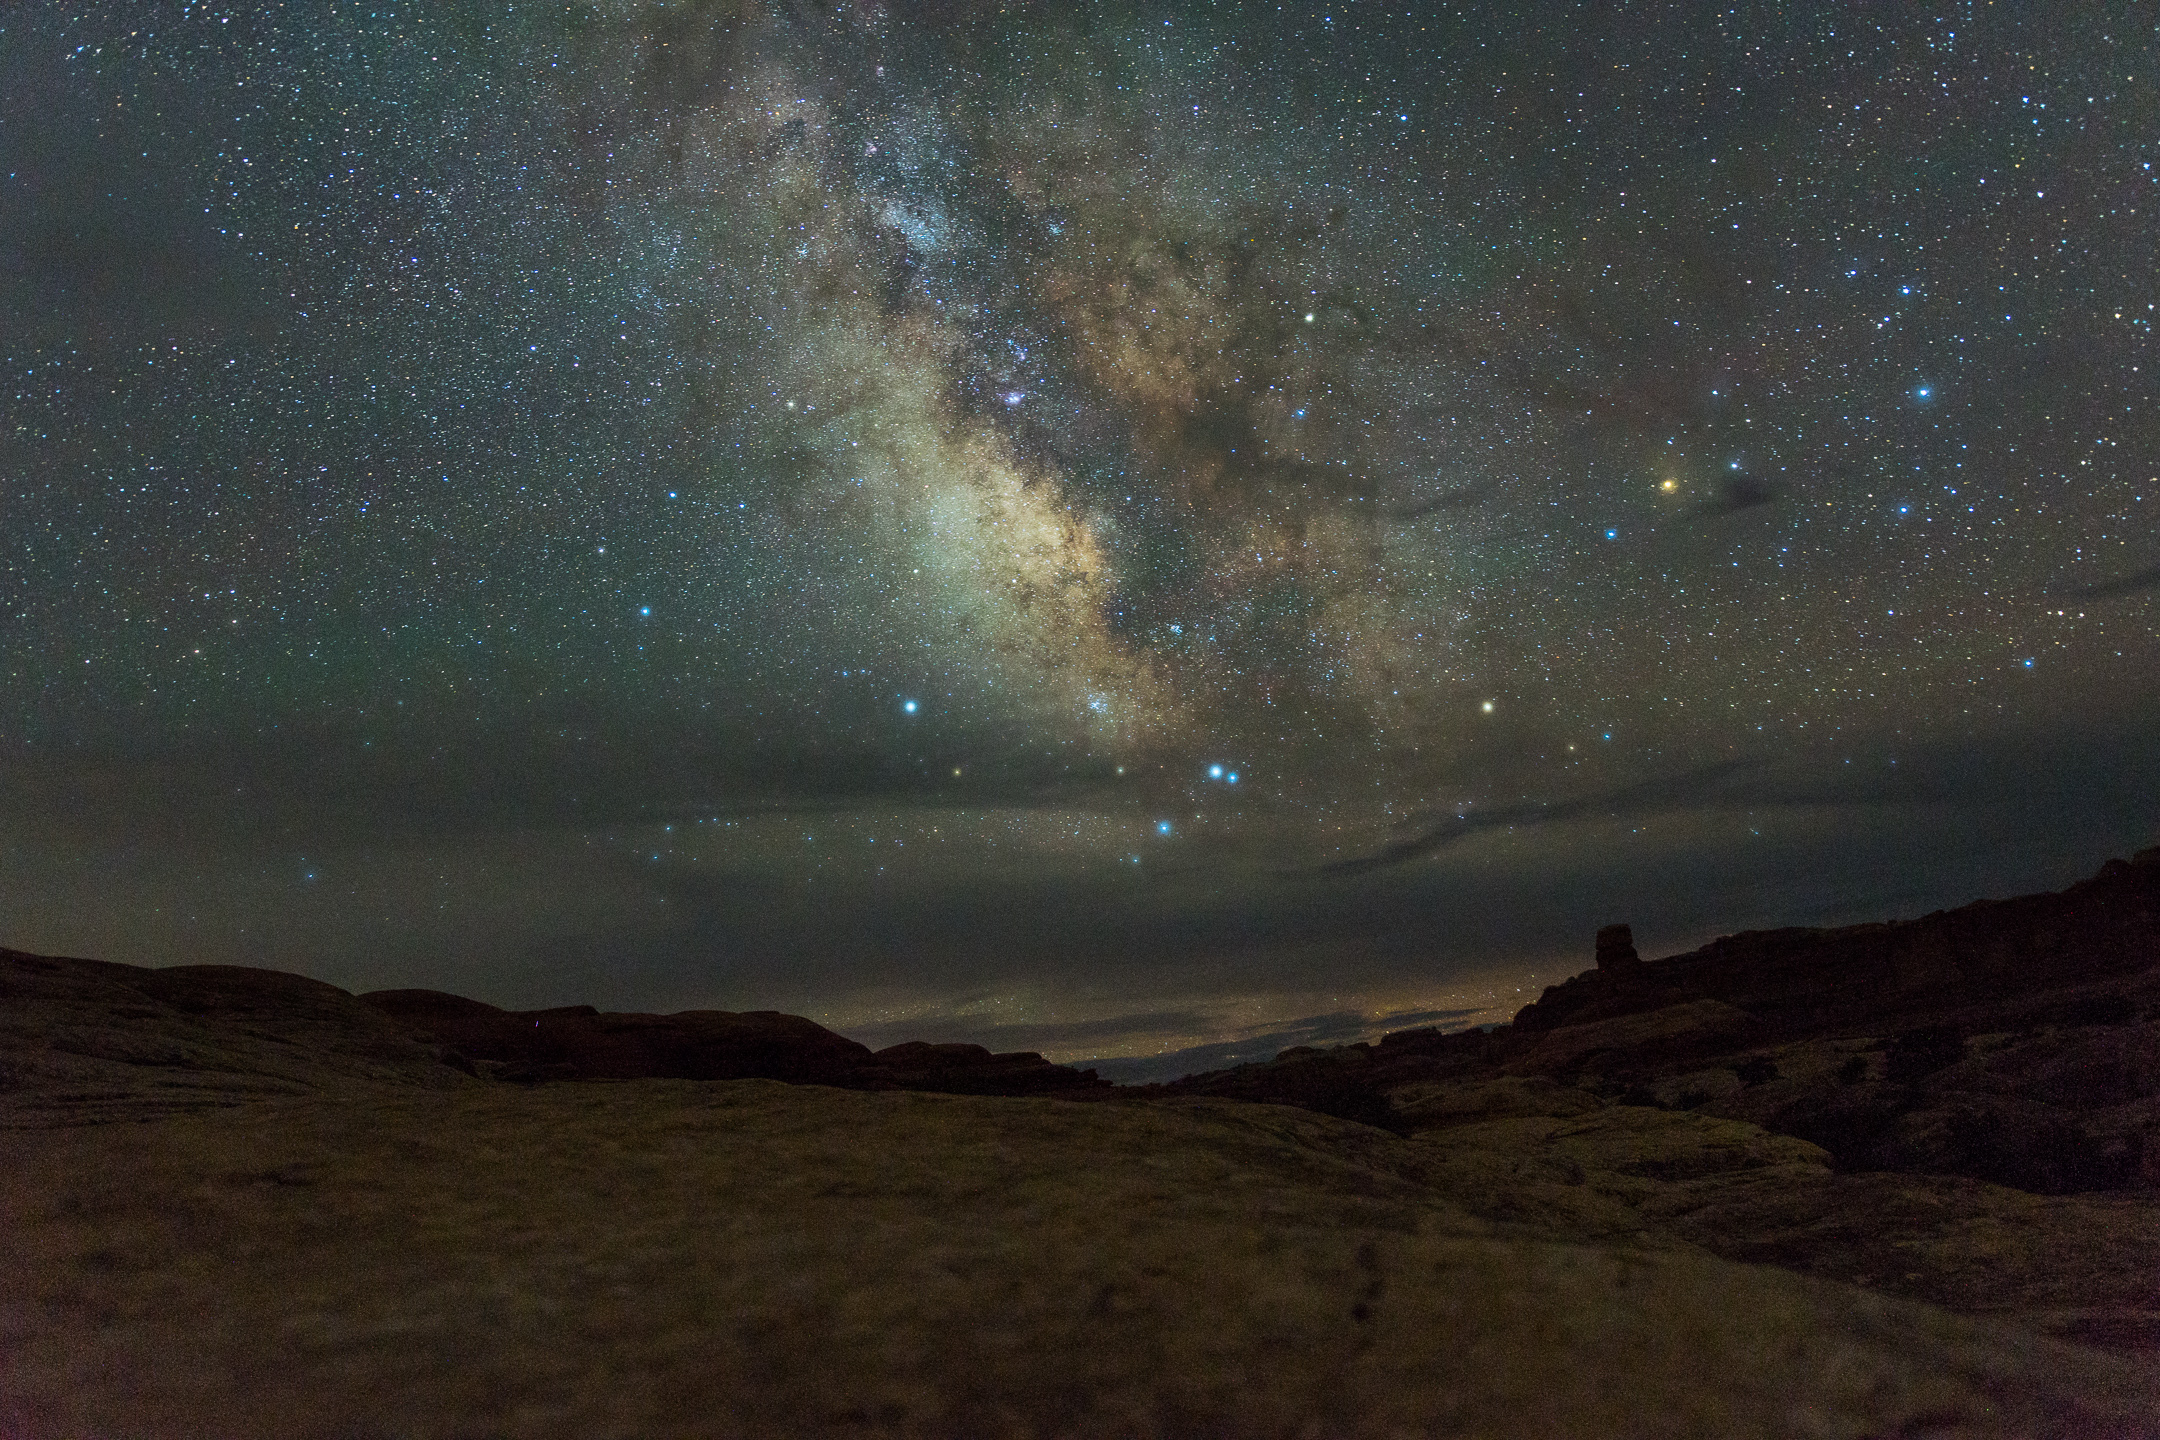
\includegraphics[width=0.9\textwidth]{canyonlands.jpg}\\
%\small{Taken about two weeks ago: ISO 6400, f/1.8, 13 seconds}\EC}

\frame{\frametitle{\textbf{Talking about the sky -- 2018's students}}
\BI
\item Chris: The sun is almost directly above my head (11:30am)
\BS\pause
\item Samantha: [The moon] was a little lower in the sky, it wasn't high in the sky just yet (9pm)
\BS\pause
\item Joseph: [The sun] was about 25\% below the horizon west, slightly south west. (7:30pm)
\BS\pause
\item Jesus: The sun was setting so it was near to the horizon... on the west. (7:30pm)
\BS\pause
\item Parker: The Moon ... was low in the sky, off to the East (10:05pm)
\BS\pause
\item Rebecca: [The Moon was] [i]n the southwest, ~80 degrees above the horizon (5am)
\BS\pause
\item Ben: The sun is currently in the South and very high in the sky (2pm)
\BS\pause
\item Petr: Sun was high up maybe one and a half palm above the horizon (6pm)
\BS\pause
\item MaryRose: [The Sun] was on my left and about a quarter of the way up into the sky (11:30am)
\BS\pause
\item Zewen: [The sun] was almost just above my head, probably a bit toward the south (I guess).
\BS\pause
\item Qianhui: The sun was at northwest ($300^\circ$) direction; the sun was rather low. By eyeballing, the sun formed a $45^\circ$ angle with the horizon. (6pm)
\BS\pause
\item Haley: The moon is visible north of the ``AXA'' building, but it's difficult to describe because if I was standing in a different location, then perhaps it would be north of the Marshall residences or North of the Carrier Dome? (11pm)
\EI
}

\frame{\frametitle{\textbf{Motion and time}}
\large
Last time we talked about the {\color{Red}distance scales} involved in astronomy.

\BS

It's also important to understand the scales in {\color{Red}time}.

\BI
\item {\color{Red}In one day} the Earth rotates around its axis.
	\pause
\item {\color{Red}In one month} the Moon orbits the Earth. 
	\pause
\item {\color{Red}In one year} the Earth orbits the Sun.
\BI
\item (It takes between a few months and a few decades for the other visible planets to orbit the Sun.)
\EI
\pause

\item {\color{Red}It takes hundreds of thousands of years} for the distant stars to move appreciably relative to us.
	\EI
}

\frame{\frametitle{\textbf{Motion and time}}

\Large
\BC
In one day, how much does the Earth move around the Sun?
\EC
\BS\BS

\color{A}A: Not at all \\
\color{B}B: Less than one degree: not enough to notice without instruments \\ 
\color{C}C: About one degree \\
\color{D}D: About ten degrees: enough that we notice it readily \\
\color{E}E: All the way around \\
}

\frame{\frametitle{\textbf{Motion and time}}

\Large
\BC
In one {\color{Red}\it{hour}}, how much does the Earth move around the Sun?
\EC
\BS\BS

\color{A}A: Not at all \\
\color{B}B: Less than one degree: not enough to notice without instruments \\ 
\color{C}C: About one degree \\
\color{D}D: About ten degrees: enough that we notice it readily \\
\color{E}E: All the way around \\
}

\frame{\frametitle{\textbf{A note on math}}

\Large\BC
The kind of math I just did is the sort of thing you'll use in this class.

\BS

I didn't do anything fancy -- just ``back-of-the-envelope'' estimation.

\BS

This kind of math is quite important in astronomy (and physics!)... 

\BS

... and it's not difficult.
\EC
}

\frame{\frametitle{\textbf{Motion and time}}

\Large
\BC
In one {\color{Red}\it{hour}}, how much does the {\color{Green}Moon} move around the Sun?
\EC
\BS\BS

\color{A}A: Not at all \\
\color{B}B: Less than one degree: not enough to notice without instruments \\ 
\color{C}C: About one degree \\
\color{D}D: About ten degrees: enough that we notice it readily \\
\color{E}E: All the way around \\

\BS\BS\pause\BC
In the course of a day, the only significant motion that happens is that the Earth turns on its axis!
\EC
}

\frame{\frametitle{\textbf{Virtual planetarium software}}
	\Large
	We can simulate the night sky tonight using {\it Stellarium} -- the program you'll need for your prelab.
	
	\bigskip
	\bigskip
	
	It's available for free on Linux, Mac OSX, and Windows.
	
	\normalsize
	
	\BI
	\item{Ubuntu users: {\tt sudo apt install stellarium}}
	\item{Fedora users: {\tt sudo dnf install stellarium}}
	\item{Windows users: see links on {\tt stellarium.org}}
	\pause\BS
	\item{Mac users: see the link on the website (not sure about M1 compatibility yet, someone tell me about this if you don't mind)}
	\EI
}






\frame{
\large

The ``celestial sphere'' model of antiquity:


\BI
\item{All the stars are attached to a sphere, very far away}
\item{This rotates around the Earth, once per day}
\EI

\bigskip\bigskip
\pause

\Large
How much of the celestial sphere can we see at a time?

\bigskip
\bigskip
\Huge
\color{A}A: All of it \\
\color{B}B: More than half  \\
\color{C}C: Half of it \\
\color{D}D: Less than half \\
\color{E}E: It depends on your latitude \\
}

\frame{\frametitle{\textbf{How good is this ``celestial sphere'' model, anyway?}}
\Large

\color{A}A: It's completely wrong; we know it's not like that! \\ 
\color{B}B: It's pretty close to correct, with a few exceptions \\
\color{C}C: It's correct, just look at the sky! \\ 
\color{D}D: It explains a lot of things, so it must have {\it some} use \\
\pause
\color{E}E: I thought Dr. Freeman was supposed to tell {\it us} this stuff?
}

\frame{\frametitle{\textbf{Problems with the celestial sphere: I}}

\Large

\BC Discuss with your neighbors: what's wrong with the celestial sphere? \EC

\pause \bigskip \bigskip

Is it really true that {\it every} star in the sky moves in the same way, all together?

\pause \bigskip \bigskip

Actually, (--------) rotates, and (--------) doesn't move much at all.

\pause\BS\BS
\small
\begin{flushright}(Lots more on this Tuesday!)\end{flushright}

}

\frame{\frametitle{\textbf{Problems with the celestial sphere: II}}

\Large

Is it really true that all the stars are stuck to a sphere, all at the same distance from us? 

\pause \bigskip \bigskip

No; we just don't have any ``depth perception'' of things this far away.
}

\frame{\frametitle{\textbf{Depth and the sky}}
\BC \Large The constellation of Orion:\EC

\begin{columns}
\begin{column}{0.5\textwidth}
\BC 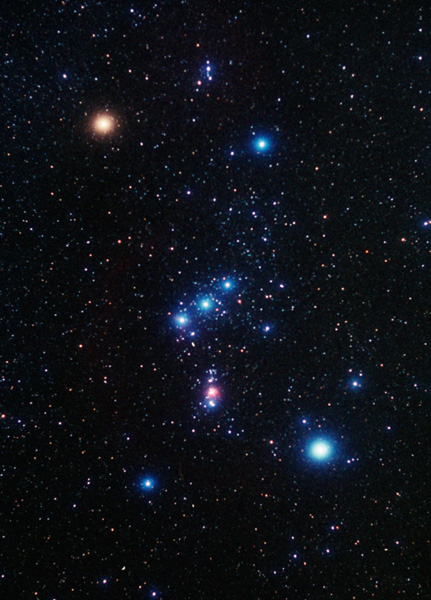
\includegraphics[width=0.8\textwidth]{orion-flat.jpg}\EC
\end{column}
\pause
\begin{column}{0.5\textwidth}
\BC 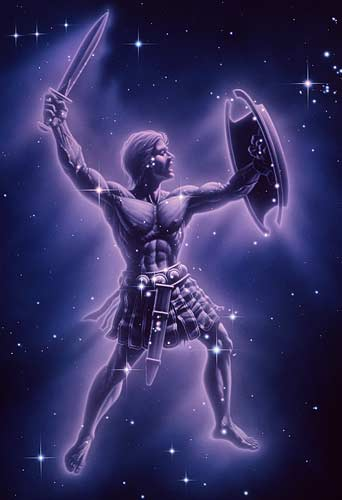
\includegraphics[width=0.8\textwidth]{orion-art.jpg}\EC
\end{column}
\end{columns}
}

\frame{\frametitle{\textbf{Depth and the sky}}
\BC \Large The reality:\EC

\bigskip
\bigskip

\BC 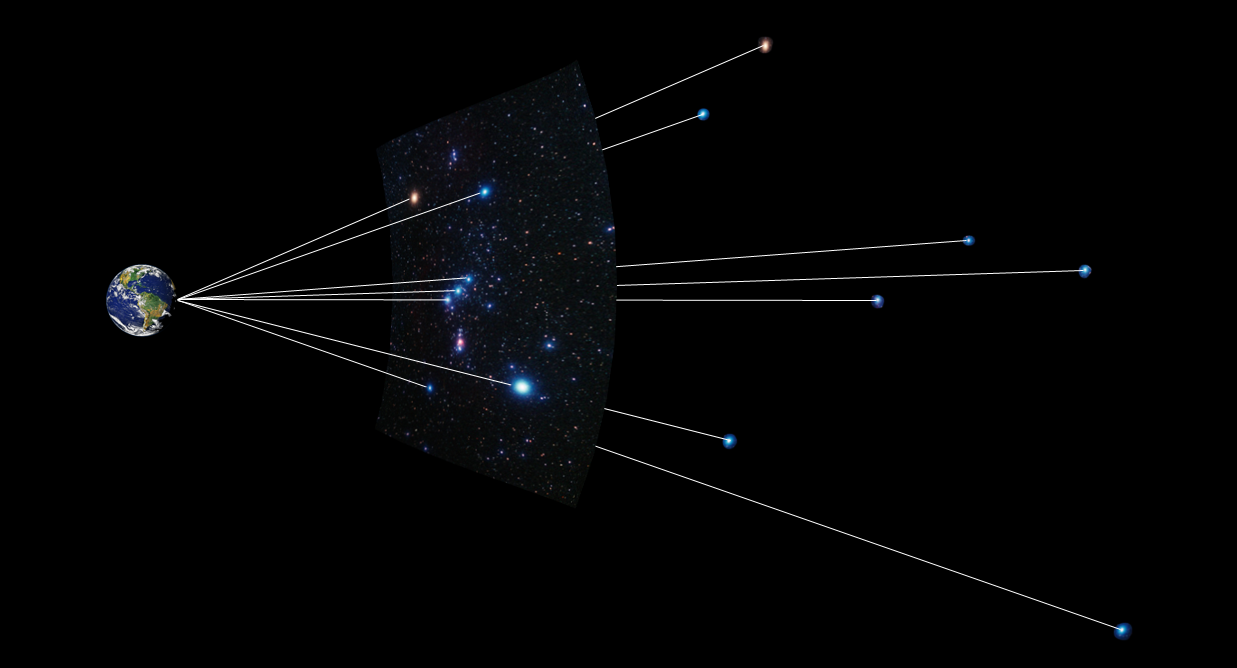
\includegraphics[width=0.9\textwidth]{orion-depth.png}\EC
}

\frame{\frametitle{\textbf{Why the celestial sphere still explains a lot}}
\Large
%Key idea \#1: the stars are {\color{Red}very far away} compared to the Earth's motion!
%\Large
%\BI
%\item{Parallax experiment: try it!}
%\pause
%\item{It doesn't matter that the stars are different distances away}
%\item{... since those distances are so huge compared to our motion}
%\pause
%\item{\color{Red}This means that the celestial sphere's predictions will be {\it badly wrong} for the motion of the Sun and the planets!}
%\EI
%
%\pause
%\bigskip
%\bigskip
%
Key idea: It doesn't matter if Earth rotates or the celestial sphere rotates: {\color{Red}relative} motion controls what we see! 

\BI
\item{The celestial sphere model is just dizzy!}
\EI
\pause
The celestial sphere model explains how the Earth's {\color{Red}} rotation affects the sky.

\BS\pause

It should thus explain the changes in the sky pretty well over {\color{Red}one day}.

\BS\pause
Over longer periods of time:
\BI
\item The Earth and the planets move around the Sun
\item The Moon moves around the Earth
\pause
\item {\bf ... so the model will need some modification for those things over longer times!}
\EI
  
}

\frame{\frametitle{\textbf{Summary}}
\large
\BI
\item{We can treat the stars as all rotating together, on an invisible sphere far away}
\item{We expect this to get the stars ``right'' and the planets and Sun ``wrong'' over longer times}
\item{The axis of rotation is the same as the Earth's, and it rotates once per day}
\item{Only half of the sphere is visible, because the Earth is in the way}
\item{{\color{Red} Horizon:} a plane lying along the Earth at our location}
\item{{\color{Red} Zenith:} the point directly overhead}
\item{{\color{Red} Celestial pole:} the point about which the stars appear to rotate}
\EI
\begin{columns}
\begin{column}{0.5\textwidth}
\BC
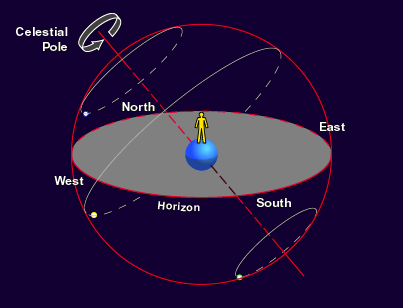
\includegraphics[width=0.8\textwidth]{sphere-1.png}\EC \end{column}
\begin{column}{0.5\textwidth}
\BC
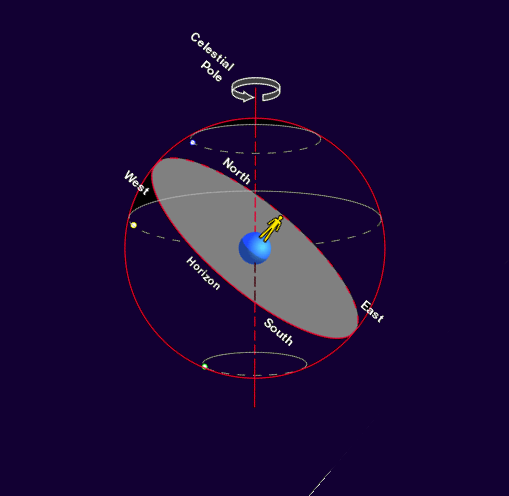
\includegraphics[width=\textwidth]{sphere-2.png}
\EC 
\end{column}
\end{columns}
}

\frame{\frametitle{\textbf{How many celestial poles are there?}}
\begin{columns}
\begin{column}{0.4\textwidth}
\Huge
\color{A}A: One \\
\color{B}B: Two \\
\color{C}C: Three \\
\color{D}D: Four 
\end{column}
\pause
\begin{column}{0.6\textwidth}
\BC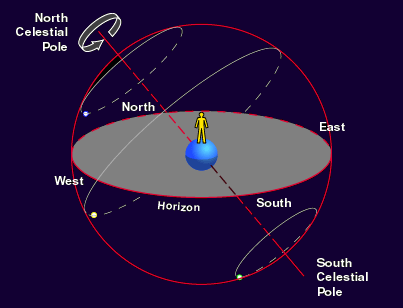
\includegraphics[width=0.8\textwidth]{sphere-3.png}\EC 
\end{column}
\end{columns}
}


\frame{\frametitle{\textbf{Lecture tutorials}}
\Huge
\BC
Complete the handout we gave you on the way in. We will do something else after this.
\EC
}

\frame{\frametitle{\textbf{Which are true in Syracuse?}}
\Large
\BI
\item{I: Some stars are always visible (at night).}
\item{II: Some stars are only visible sometimes; they rise and set during the night}
\item{III: Some stars are never visible}
\EI

\bigskip
\bigskip

\color{A}A: I only \\
\color{B}B: II only \\
\color{C}C: III only \\
\color{D}D: I and II \\
\color{E}E: I, II, and III 
}

\frame{\frametitle{\textbf{Summary}}
	\large
	\BI
	\item{We can treat the stars as all rotating together, on an invisible sphere far away}
	\item{We expect this to get the stars ``right'' and the planets and Sun ``wrong''}
	\item{The axis of rotation is the same as the Earth's, and it rotates once per day}
	\item{Only half of the sphere is visible, because the Earth is in the way}
	\item{{\color{Red} Horizon:} a plane lying along the Earth at our location}
	\item{{\color{Red} Zenith:} the point directly overhead}
	\item{{\color{Red} Celestial poles:} the points about which the stars appear to rotate}
	\EI
	\BC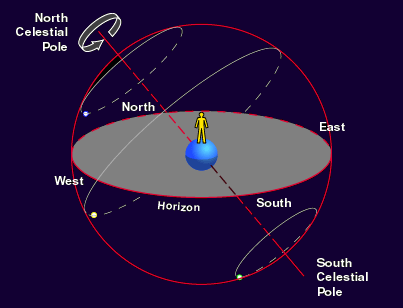
\includegraphics[width=0.5\textwidth]{sphere-3.png}\EC 
}


\frame{\frametitle{\textbf{What is this?}}
\BC
\includegraphics[width=0.6\textwidth]{aus-flag.png}\EC

\pause

\Large \BC The Australian flag, with a pattern of stars called the Southern Cross.

These stars are only visible in the Southern Hemisphere!
\EC
}


\end{document}
